\begin{center}\section{向量}\label{chapter_vector}\end{center}
\subsection{向量的概念}
\begin{minipage}{.7\textwidth}
	\begin{align*}
		\mbox{向量:}&\mbox{既有大小又有方向的量}\\
		\mbox{向量表示:}&\overrightarrow{AB}\ \mbox{或}\ \overrightarrow{a}\\
		\mbox{自由向量:}&\mbox{与起点无关的向量}\\
		\mbox{向量的模:}&|\overrightarrow{AB}|\quad|\overrightarrow{a}|\\
		\mbox{单位向量:}&|\overrightarrow{a}|=1\\
		\overrightarrow{a}\mbox{单位向量:}&\begin{cases}
			\overrightarrow{e}_{\overrightarrow{a}}=\frac{\overrightarrow{a}}{|\overrightarrow{a}|}=\frac{1}{|\overrightarrow{a}|}\overrightarrow{a}\\
			\overrightarrow{a}=|\overrightarrow{a}|\overrightarrow{e}_{\overrightarrow{a}}
		\end{cases}\\
		\overrightarrow{0}\mbox{向量:}&\begin{cases}
			|\overrightarrow{a}|=0\mbox{记作:}\overrightarrow{a}=\overrightarrow{0}\mbox{方向任意}\\
			\overrightarrow{0}\mbox{与任何向量平行}\\
			\overrightarrow{0}\mbox{与任何向量垂直}
		\end{cases}\\
		\mbox{向量夹角:}&0\leqslant\varphi\leqslant \pi\quad (\overrightarrow{a}\textasciicircum\overrightarrow{b})=\varphi\\
		\mbox{向量平行:}&\overrightarrow{a}//\overrightarrow{b}\Leftrightarrow\begin{cases}
			(\overrightarrow{a}\textasciicircum\overrightarrow{b})=0\mbox{或}(\overrightarrow{a}\textasciicircum\overrightarrow{b})=\pi\\
			\overrightarrow{a}=\lambda \overrightarrow{b}\quad(\mbox{存在唯一}\lambda)
		\end{cases}\\
		\mbox{向量平行:}&\overrightarrow{a}\perp\overrightarrow{b}\mbox{或}(\overrightarrow{a}\textasciicircum\overrightarrow{b})=\frac{\pi}{2}
	\end{align*}
\subsection{向量的线性运算}
	$\mbox{三角不等式:}\begin{cases}
	|\overrightarrow{a}+\overrightarrow{b}|\leqslant|\overrightarrow{a}|+|\overrightarrow{b}|\\
	|\overrightarrow{a}-\overrightarrow{b}|\leqslant|\overrightarrow{a}|+|\overrightarrow{b}|
\end{cases}$\\
	$\mbox{向量的加法:}\begin{cases}
		\overrightarrow{a}+\overrightarrow{b}\\
		\mbox{交换律:}\overrightarrow{a}+\overrightarrow{b}=\overrightarrow{b}+\overrightarrow{a}\\
		\mbox{结合律:}(\overrightarrow{a}+\overrightarrow{b})+\overrightarrow{c}=\overrightarrow{a}+(\overrightarrow{b}+\overrightarrow{v})
	\end{cases}$\\
	$\mbox{向量的减法:}\begin{cases}
		\mbox{负向量:}\mbox{与}\overrightarrow{a}\mbox{大小相等方向相反的向量}-\overrightarrow{a}\\
		\overrightarrow{b}-\overrightarrow{a}=\overrightarrow{b}+(-\overrightarrow{a})\\
		\overrightarrow{a}-\overrightarrow{a}=\overrightarrow{0}\\
		\overrightarrow{AB}=\overrightarrow{OB}-\overrightarrow{OA}
	\end{cases}$
\end{minipage}
\hfill
\begin{minipage}{.3\textwidth}
	\begin{center}
		\begin{tikzpicture}[>=latex]
			\draw[->](0,0)node[below]{$A$}--(2,1)node[above]{$B$};
		\end{tikzpicture}\\
		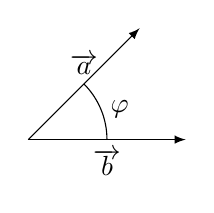
\begin{tikzpicture}[>=latex]
			\draw[->](0,0)--node[above]{$\overrightarrow{a}$}(45:2);
			\draw[->](0,0)--node[below]{$\overrightarrow{b}$}(2,0);
			\draw(1,0) arc (0:45:1);
			\node at (22.5:1)[right]{$\varphi$};
		\end{tikzpicture}\\
			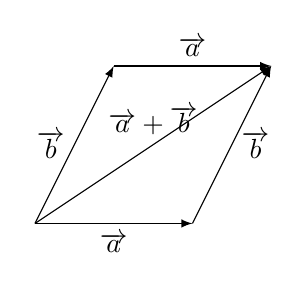
\begin{tikzpicture}[>=latex]
		\draw[->](0,0)--node[above]{$\overrightarrow{a}+\overrightarrow{b}$}(3,2);
		\draw[->](0,0)--node[below]{$\overrightarrow{a}$}(2,0);
		\draw[->](1,2)--node[above]{$\overrightarrow{a}$}(3,2);
		\draw[->](2,0)--node[right]{$\overrightarrow{b}$}(3,2);
		\draw[->](0,0)--node[left]{$\overrightarrow{b}$}(1,2);
	\end{tikzpicture}\\
	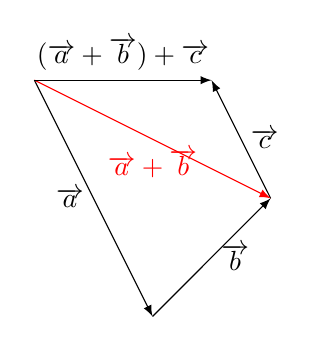
\begin{tikzpicture}[>=latex,scale=1.5]
	\draw[->] (0,2)coordinate (A)--node[left]{$\overrightarrow{a}$}(1,0)coordinate (B);
	\draw[->] (B)--node[right]{$\overrightarrow{b}$}(2,1)coordinate (C);
	\draw[->] (C)--node[right]{$\overrightarrow{c}$}(1.5,2)coordinate (D);
	\draw[->,color=red] (A)--node[below]{$\overrightarrow{a}+\overrightarrow{b}$}(C);
	\draw[->] (A)--node[above]{$(\overrightarrow{a}+\overrightarrow{b})+\overrightarrow{c}$}(D);
\end{tikzpicture}\\
	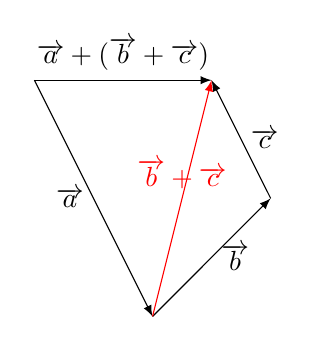
\begin{tikzpicture}[>=latex,scale=1.5]
	\draw[->] (0,2)coordinate (A)--node[left]{$\overrightarrow{a}$}(1,0)coordinate (B);
	\draw[->] (B)--node[right]{$\overrightarrow{b}$}(2,1)coordinate (C);
	\draw[->] (C)--node[right]{$\overrightarrow{c}$}(1.5,2)coordinate (D);
	\draw[->,color=red] (B)--node[above]{$\overrightarrow{b}+\overrightarrow{c}$}(D);
	\draw[->] (A)--node[above]{$\overrightarrow{a}+(\overrightarrow{b}+\overrightarrow{c})$}(D);
\end{tikzpicture}\\
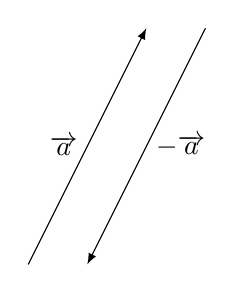
\begin{tikzpicture}[>=latex,scale=1.5]
	\draw[->] (0,0)--node[left]{$\overrightarrow{a}$}(1,2);
	\draw[<-] (.5,0)--node[right]{$-\overrightarrow{a}$}(1.5,2);
\end{tikzpicture}
	\end{center}
\end{minipage}
\mbox{向量的数乘:}$\begin{cases}
	\mbox{大小:}|\lambda \overrightarrow{a}|=|\lambda||\overrightarrow{a}|\\
	\mbox{方向:}\begin{cases}
		\lambda>0\quad\mbox{时}\lambda\overrightarrow{a}\mbox{与}\overrightarrow{a}\mbox{方向一致}\\
		\lambda<0\quad\mbox{时}\lambda\overrightarrow{a}\mbox{与}\overrightarrow{a}\mbox{方向相反不}
	\end{cases}\\
\mbox{特殊数相乘:}\begin{cases}
	0\mbox{:}0\overrightarrow{a}=\overrightarrow{0}\\
	1\mbox{:}1\overrightarrow{a}=\overrightarrow{a}\\
	-1\mbox{:}(-1)\overrightarrow{a}=-\overrightarrow{a}
\end{cases}\\
\mbox{交换律:}\lambda(\mu\overrightarrow{a})=(\lambda\mu)\overrightarrow{a}=\mu(\lambda\overrightarrow{a})\\
\mbox{结合律:}\begin{cases}
	(\lambda+\mu)\overrightarrow{a}=\lambda\overrightarrow{a}+\mu\overrightarrow{a}\\
	\lambda(\overrightarrow{a}+\overrightarrow{b})=\lambda\overrightarrow{a}+\lambda\overrightarrow{b}
\end{cases}
\end{cases}$
\subsection{空间直角坐标系}
\begin{minipage}{.6\textwidth}
	\begin{align*}
		\mbox{坐标原点:}&O\\
		\mbox{坐标轴:}&\begin{cases}
			x\mbox{轴}\quad\mbox{单位向量}\overrightarrow{i}\\
			y\mbox{轴}\quad\mbox{单位向量}\overrightarrow{j}\\
			z\mbox{轴}\quad\mbox{单位向量}\overrightarrow{k}
		\end{cases}\\
		\mbox{坐标面:}&x\circ y\mbox{面}\ y\circ z\mbox{面}\ z\circ x\mbox{面}\\
		\mbox{坐标向量运算:}&\begin{cases}
			\overrightarrow{a}=(a_x,a_y,a_z)\quad\overrightarrow{b}=(b_x,b_y,b_z)\\
			\overrightarrow{a}+\overrightarrow{b}=(a_x+b_x,a_y+b_y,a_z+b_z)\\
			\overrightarrow{a}-\overrightarrow{b}=(a_x-b_x,a_y-b_y,a_z-b_z)\\
			\lambda\overrightarrow{a}=(\lambda a_x,\lambda a_y,\lambda a_z)
		\end{cases}
	\end{align*}
\end{minipage}
\hfill
\begin{minipage}{.4\textwidth}
	\begin{center}
		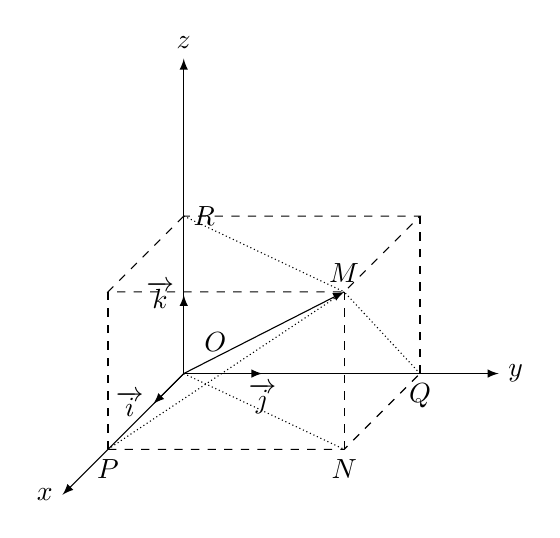
\begin{tikzpicture}[>=latex,scale=1]
			%(y,z,x)
			\node at (.4,.4,0)[]{$O$};
			\draw[->] (0,0,0)--(1,0,0)node[below]{$\overrightarrow{j}$};
			\draw[->] (0,0,0)--(0,0,1)node[left]{$\overrightarrow{i}$};
			\draw[->] (0,0,0)--(0,1,0)node[left]{$\overrightarrow{k}$};
			\draw[->] (0,0,0)--(4,0,0)node[right]{$y$};
			\draw[->] (0,0,0)--(0,0,4)node[left]{$x$};
			\draw[->] (0,0,0)--(0,4,0)node[above]{$z$};
			\draw[->] (0,0,0)--(3,2,2.5)node[above]{$M$};
			\draw[dashed] (0,0,2.5)node[below]{$P$}--(3,0,2.5)node[below]{$N$}--(3,0,0)node[below]{$Q$};
			\draw[dashed] (0,2,0)node[right]{$R$}--(0,2,2.5)--(3,2,2.5)--(3,2,0)--cycle;
			\draw[dashed](0,0,2.5)--(0,2,2.5);
			\draw[dashed](3,0,2.5)--(3,2,2.5);
			\draw[dashed](3,0,0)--(3,2,0);
			\draw[densely dotted](0,0,0)--(3,0,2.5);
			\draw[densely dotted](0,0,2.5)--(3,2,2.5);
			\draw[densely dotted](0,2,0)--(3,2,2.5);
			\draw[densely dotted](3,0,0)--(3,2,2.5);
		\end{tikzpicture}
	\end{center}
\end{minipage}
$$\mbox{方向角:}\begin{cases}
	x\mbox{轴}\quad \cos\alpha=\frac{x}{|\overrightarrow{OM}|}=\frac{x}{\sqrt{x^2+y^2+z^2}}\\
	y\mbox{轴}\quad \cos\beta=\frac{y}{|\overrightarrow{OM}|}=\frac{y}{\sqrt{x^2+y^2+z^2}}\\
	z\mbox{轴}\quad \cos\gamma=\frac{z}{|\overrightarrow{OM}|}=\frac{z}{\sqrt{x^2+y^2+z^2}}
\end{cases}\quad
\mbox{投影:}\begin{cases}
	x\mbox{轴}\ \mbox{记:} Prj_{x}^{\ \overrightarrow{OM}}=|\overrightarrow{OM}|\cos\alpha\\
	y\mbox{轴}\ \mbox{记:}Prj_{y}^{\ \overrightarrow{OM}}=|\overrightarrow{OM}|\cos\beta\\
	z\mbox{轴}\ \mbox{记:}Prj_{z}^{\ \overrightarrow{OM}}=|\overrightarrow{OM}|\cos\gamma
\end{cases}$$
	\begin{align}
	M\mbox{点坐标}(x,y,z)\Leftrightarrow\overrightarrow{OM}=x\overrightarrow{i}+y\overrightarrow{j}+z\overrightarrow{k}\label{Coordinate_representation_1}
\end{align}
\begin{align}
	|\overrightarrow{OM}|=\sqrt{x^2+y^2+z^2}\label{Coordinate_representation_2}
\end{align}
\begin{align}
A(x_1,y_1,z_1)\quad B(x_2,y_2,z_2)\quad |AB|=|\overrightarrow{AB}|=\sqrt{(x_2-x_1)^2,(y_2-y_1)^2,(z_2-z_1)^2}\label{Coordinate_representation_3}
\end{align}
\begin{equation}
	(\cos\alpha,\cos\beta,\cos\gamma)=\frac{\overrightarrow{OM}}{|\overrightarrow{OM}|}=\overrightarrow{e}_{\overrightarrow{OM}}\label{Coordinate_representation_4}
\end{equation}
\begin{equation}
	\cos^2\alpha+\cos^2\beta+\cos^2\gamma=1\label{Coordinate_representation_5}
\end{equation}
$$\mbox{投影定义}Prj_{\overrightarrow{u}}^{\ \overrightarrow{a}}=|\overrightarrow{a}|\cos(\overrightarrow{a}\textasciicircum\overrightarrow{u})$$
\begin{align}
	Prj_{\overrightarrow{u}}^{\ (\overrightarrow{a}+\overrightarrow{b})}&=Prj_{\overrightarrow{u}}^{\ \overrightarrow{a}}+Prj_{\overrightarrow{u}}^{\ \overrightarrow{b}}\\
	Prj_{\overrightarrow{u}}^{\ \lambda\overrightarrow{a}}&=\lambda Prj_{\overrightarrow{u}}^{\ \overrightarrow{a}}
\end{align}
\subsection{数量积,向量积,混合积}
$$\mbox{数量积(内积)}:\ \overrightarrow{a}\bullet\overrightarrow{b}\triangleq|\overrightarrow{a}||\overrightarrow{b}|\cos(\overrightarrow{a}\textasciicircum\overrightarrow{b})\begin{cases}
	\overrightarrow{a}\bullet\overrightarrow{b}=|\overrightarrow{a}|	Prj_{\overrightarrow{a}}^{\ \overrightarrow{b}}=|\overrightarrow{b}|Prj_{\overrightarrow{b}}^{\ \overrightarrow{a}}\\
	\overrightarrow{a}\bullet\overrightarrow{a}=|\overrightarrow{a}|^2\\
	\overrightarrow{a}\perp\overrightarrow{b}\Leftrightarrow\overrightarrow{a}\bullet\overrightarrow{b}=0\\
	\overrightarrow{a}\bullet\overrightarrow{b}=\overrightarrow{b}\bullet\overrightarrow{a}\quad(\mbox{交换律})\\
	(\lambda\overrightarrow{a})\bullet\overrightarrow{b}=\overrightarrow{a}\bullet(\lambda\overrightarrow{b})\\
	(\overrightarrow{a}+\overrightarrow{b})\bullet\overrightarrow{c}=\overrightarrow{a}\bullet\overrightarrow{c}+\overrightarrow{b}\bullet\overrightarrow{c}\quad\mbox{分配律}\\
\end{cases}$$
\begin{align}
	\mbox{坐标表达式:}\overrightarrow{a}\bullet\overrightarrow{b}=a_xb_x+a_yb_y+a_zb_z\label{Inner_product_coordinate}
\end{align}
$$\mbox{向量积}:\ |\overrightarrow{a}\times\overrightarrow{b}|\triangleq|\overrightarrow{a}||\overrightarrow{b}|\sin(\overrightarrow{a}\textasciicircum\overrightarrow{b})\begin{cases}
	\overrightarrow{a}\times\overrightarrow{a}=0\\
	\overrightarrow{a}//\overrightarrow{b}\Leftrightarrow\overrightarrow{a}\times\overrightarrow{b}=0\\
	\overrightarrow{a}\times\overrightarrow{b}=-\overrightarrow{b}\times\overrightarrow{a}\\
	(\lambda\overrightarrow{a})\times\overrightarrow{b}=\overrightarrow{a}\times(\lambda\overrightarrow{b})\\
	(\overrightarrow{a}+\overrightarrow{b})\times\overrightarrow{c}=\overrightarrow{a}\times\overrightarrow{c}+\overrightarrow{b}\times\overrightarrow{c}\\	\overrightarrow{a}\times(\overrightarrow{b}+\overrightarrow{c})=\overrightarrow{a}\times\overrightarrow{b}+\overrightarrow{a}\times\overrightarrow{c}\\
\end{cases}$$
$$\overrightarrow{a}\times\overrightarrow{b}\mbox{是垂直与两个向量的向量,右手a到b,大拇指指的方向}$$
\begin{minipage}{.7\textwidth}
\begin{align}
	\overrightarrow{a}\times\overrightarrow{b}=\begin{vmatrix}
		a_y & a_z\\
		b_y & b_z
	\end{vmatrix}\overrightarrow{i}-\begin{vmatrix}
		a_x & a_z\\
		b_x & b_z
	\end{vmatrix}\overrightarrow{j}+\begin{vmatrix}
		a_x & a_y\\
		b_x & b_y
	\end{vmatrix}\overrightarrow{k}\label{Vector_product_coordinate}
\end{align}
\end{minipage}
\hfill
\begin{minipage}{.3\textwidth}
$$\begin{vmatrix}
	\overrightarrow{i} & \overrightarrow{j} & \overrightarrow{k}\\
	a_x & a_y & a_z\\
	b_x & b_y & b_z
\end{vmatrix}$$
\end{minipage}\\
\par
\begin{minipage}{.7\textwidth}
$$\mbox{混合积:}(\overrightarrow{a}\times\overrightarrow{b})\bullet\overrightarrow{c}=\begin{vmatrix}
	a_y & a_z\\
	b_y & b_z
\end{vmatrix}c_x-\begin{vmatrix}
	a_x & a_z\\
	b_x & b_z
\end{vmatrix}c_y+\begin{vmatrix}
	a_x & a_y\\
	b_x & b_y
\end{vmatrix}c_z$$
\end{minipage}
\hfill
\begin{minipage}{.3\textwidth}
$$\begin{vmatrix}
	c_x & c_y & c_z\\
	a_x & a_y & a_z\\
	b_x & b_y & b_z
\end{vmatrix}$$
\end{minipage}
\subsection{空间曲面及其方程}
\subsubsection{概念}
$$F(x,y,z)=0$$
\mbox{与平面垂直的非零向量称为法向量}\\
\subsubsection{平面表达式}
$$\mbox{法向量}\overrightarrow{n}=(A,B,C)\ \mbox{平面$\pi$上一点}P_0(x_0,y_0,z_0),M(x,y,z)\mbox{为平面$\pi$上任意点}$$
\begin{align*}
	\mbox{平面点法式:}&A(x-x_0)+B(y-y_0)+C(z-z_0)=0\\
	\mbox{平面截距式:}&\frac{x}{a}+\frac{y}{b}+\frac{z}{c}=1\\
	\mbox{平面一般方程:}&Ax+By+Cz+D=0\begin{cases}
		D=0\Leftrightarrow \pi\mbox{过原点}\\
		A=0\Leftrightarrow \overrightarrow{n}\perp x\mbox{轴}\Leftrightarrow \pi// x\mbox{轴}\\
		B=0\Leftrightarrow \pi// y\mbox{轴}\\
		C=0\Leftrightarrow \pi// z\mbox{轴}\\
		A=0,B=0\Leftrightarrow \pi// x\circ y\mbox{面}
	\end{cases}
\end{align*}
\subsubsection{平面夹角}
\begin{align*}
	A_1x+B_1y+C_1z+D_1=0\qquad \overrightarrow{n_1}=(A_1,B_1,C_1)\\
	A_2x+B_2y+C_2z+D_2=0\qquad \overrightarrow{n_2}=(A_2,B_2,C_2)\\
	\cos\theta=\frac{|\overrightarrow{n_1}\bullet\overrightarrow{n_2}|}{|\overrightarrow{n_1}|\bullet|\overrightarrow{n_2}|}=\frac{|A_1A_2+B_1B_2+C_1C_2|}{\sqrt{A_1^2+B_1^2+C_1^2}\sqrt{A_2^2+B_2^2+C_2^2}}
\end{align*}
\subsubsection{点到平面距离}
$$\mbox{平面}\pi:\quad Ax+By+Cz+D=0\ \mbox{平面外一点}P_0(x_0,y_0,z_0)$$\\
$$|P_0N|=\left|Prj_{\overrightarrow{n}}^{\ \overrightarrow{P_1P_0}}\right|=\frac{\left|\overrightarrow{n}\bullet\overrightarrow{P_1P_0}\right|}{|\overrightarrow{n}|}=\frac{|Ax_0+By_0+Cz_0+D|}{\sqrt{A^2+B^2+C^2}}$$
\subsection{空间线及其方程}
\subsubsection{曲线的一般方程}
$$\mbox{一般方程}\begin{cases}
	F(x,y,z)=0\\
	G(x,y,z)=0
\end{cases}$$
\subsubsection{直线的一般方程}
\begin{align*}
	\mbox{一般方程:}&\begin{cases}
		A_1x+B_1y+C_1z+D_1=0\\
		A_2x+B_2y+C_2z+D_2=0
	\end{cases}\\
	\mbox{对称式:}&\frac{x-x_0}{m}=\frac{y-y_0}{n}=\frac{z-z_0}{p}=t\begin{cases}
		\overrightarrow{M_0M}=(x-x_0,y-y_0,z-z_0)\\
		\mbox{方向量}\overrightarrow{S}=(m,n,p)
	\end{cases}\\
	\mbox{参数方程:}&\begin{cases}
		x=x_0+mt\\
		y=y_0+mt\\
		z=z_0+mt
	\end{cases}
\end{align*}
\subsubsection{两直线夹角}
两直线的方向向量的夹角称为两直线的夹角(要求为锐角)\\
$L_1:\ \mbox{方向向量}\overrightarrow{S_1}=(m_1,n_1,p_1)$\\
$L_2:\ \mbox{方向向量}\overrightarrow{S_2}=(m_2,n_2,p_2)$\\
$L_1\mbox{与}L_2\mbox{的夹角}(\overrightarrow{S_1}\textasciicircum\overrightarrow{S_2})\quad(\overrightarrow{S_1}\textasciicircum-\overrightarrow{S_2})$
$$\cos\varphi=\frac{|\overrightarrow{S_1}\bullet\overrightarrow{S_2}|}{|\overrightarrow{S_1}||\overrightarrow{S_2}|}=\frac{|m_1m_2+n_1n_2+p_1p_2|}{\sqrt{m_1^2+n_1^2+p_1^2}\sqrt{m_2^2+n_2^2+p_2^2}}$$
\subsubsection{线与面夹角}
$L:\ \mbox{方向向量}\overrightarrow{S}=(m,n,p)$\\
$\pi:\ \mbox{法向量}\overrightarrow{n}=(A,B,C)$\\
$$\cos\theta=\frac{|\overrightarrow{S}\bullet\overrightarrow{n}|}{|\overrightarrow{S}||\overrightarrow{n}|}=\frac{|Am+Bn+Cp|}{\sqrt{A^2+B^2+C^2}\sqrt{m^2+n^2+p^2}}$$
$$\sin\varphi=\cos(\frac{\pi-\theta}{2})$$